%\title{CWLT Review Session Poster}
\documentclass[12pt,letterpaper]{article}

\title{Poster Template}

\usepackage{hyperref}
\usepackage{setspace}
\usepackage{amsmath}%
\usepackage{MnSymbol}%
\usepackage{wasysym}%
\usepackage{lmodern}


\usepackage[utf8]{inputenc}
\usepackage[T1]{fontenc}
\usepackage[sfdefault,lf]{carlito}

\usepackage[margin=1.1cm,letterpaper]{geometry}
\usepackage{multicol}
\usepackage{ragged2e}
\usepackage{tabularx}
\usepackage[table]{xcolor}
\usepackage{graphicx}

%cyan 36a8b8
%blue b2d4ef
%purple c677dd
%overleaf green 4F9C45
%green 7b9e62
%red 1 cb4752
%red 2 be5046
%orange 1 d19a66
%orange 2 e5c07b

\definecolor{HighlightColor}{HTML}{c677dd}
\graphicspath{{img/}}
\pagestyle{empty}
\RaggedRight
\parskip=12pt plus 4pt

\begin{document}


{\fontsize{40pt}{42pt}\bfseries\selectfont\color{HighlightColor}%
Calculus Now, Summer Soon
\\}% 
%\begin{flushright}
~\hfill
{\LARGE\bfseries%
\mbox{1pm Sun May 7 and 1pm Mon May 8 @ CWLT (Howarth 109)}%
}

\vspace{-2ex}


\begin{large}
\justify
{\Large You're excited for summer, but you've got one last hurdle to clear: your final calculus exam.

\noindent
Get some extra help and study time at the CWLT! Come to one (or both) of the Math 180 and 181 review sessions led by math tutors Henry and Matthew. 

\noindent
It will be summer soon. We'll help you get there!\par}

\end{large}

%

{\centering%
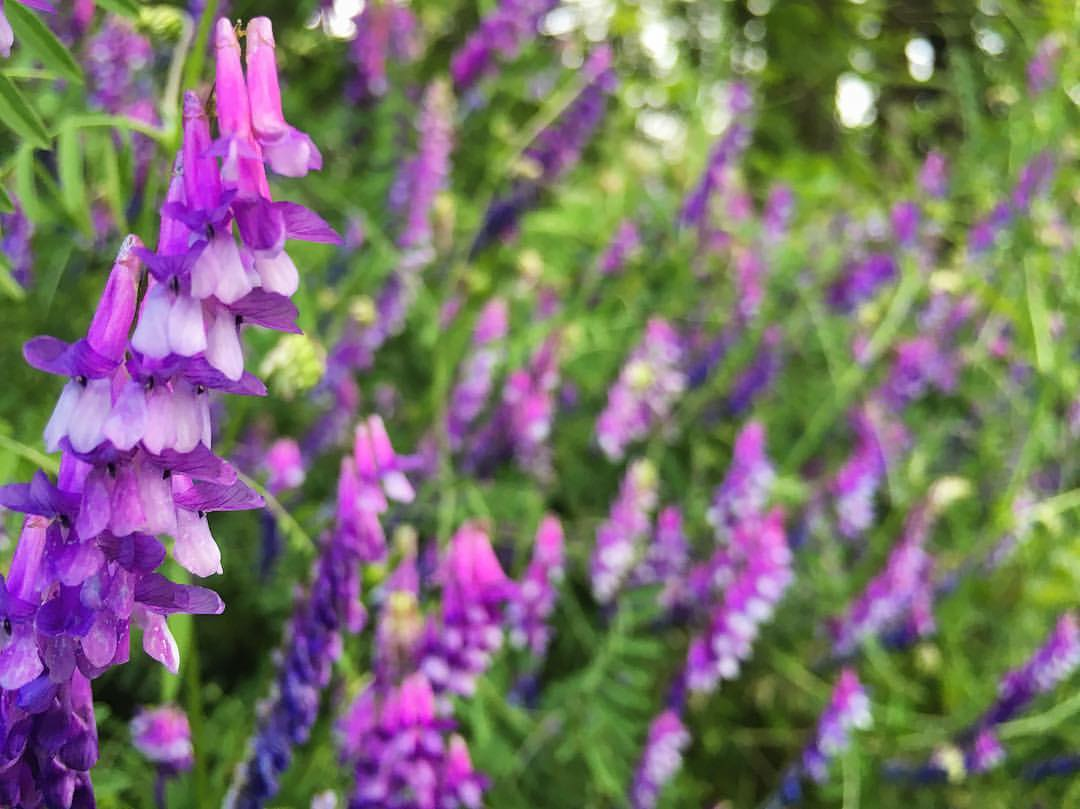
\includegraphics[width=\linewidth,trim={0 0 5cm 0},clip]{summer_flowers}%
\par}

\vfill

{\LARGE Center for Writing, Learning, \& Teaching}
\hfill
{\LARGE \url{pugetsound.edu/cwlt}}
\end{document}